\documentclass[12pt]{article}
\usepackage{graphicx}
\usepackage[margin=2cm]{geometry}
\usepackage[utf8]{inputenc}
\usepackage{tikz}
\usepackage[export]{adjustbox}
\usepackage{indentfirst}
\usepackage{wrapfig}
\usepackage{listings}
\usepackage{color}
\usepackage{enumerate}
\usepackage{amssymb, bm}
\usepackage{csvsimple}
\usepackage{tikz}
\usetikzlibrary{positioning}
\usepackage{lscape}
\usepackage{amsmath}
\newcommand\tab[1][1cm]{\hspace*{#1}}
\definecolor{mygreen}{rgb}{0,0.6,0}
\definecolor{mygray}{rgb}{0.5,0.5,0.5}
\definecolor{mymauve}{rgb}{0.58,0,0.82}
\lstset{ %
    backgroundcolor=\color{gray!10!white},
  basicstyle=\tiny, %footnotesize,        % the size of the fonts that are used for the code
  breakatwhitespace=false,         % sets if automatic breaks should only happen at whitespace
  breaklines=true,                 % sets automatic line breaking
  captionpos=b,                    % sets the caption-position to bottom
  commentstyle=\color{mygreen},    % comment style
  deletekeywords={...},            % if you want to delete keywords from the given language
  escapeinside={\%*}{*)},          % if you want to add LaTeX within your code
  extendedchars=true,              % lets you use non-ASCII characters; for 8-bits encodings only, does not work with UTF-8
  frame=single,	                   % adds a frame around the code
  keepspaces=true,                 % keeps spaces in text, useful for keeping indentation of code (possibly needs columns=flexible)
  keywordstyle=\color{blue},       % keyword style
  language=Python,                 % the language of the code
  morekeywords={*,...},           % if you want to add more keywords to the set
  numbers=left,                    % where to put the line-numbers; possible values are (none, left, right)
  numbersep=10pt,                   % how far the line-numbers are from the code
  numberstyle=\tiny\color{mygray}, % the style that is used for the line-numbers
  rulecolor=\color{black},         % if not set, the frame-color may be changed on line-breaks within not-black text (e.g. comments (green here))
  showspaces=false,                % show spaces everywhere adding particular underscores; it overrides 'showstringspaces'
  showstringspaces=false,          % underline spaces within strings only
  showtabs=false,                  % show tabs within strings adding particular underscores
  stepnumber=1,                    % the step between two line-numbers. If it's 1, each line will be numbered
  stringstyle=\color{mymauve},     % string literal style
  tabsize=1,	                   % sets default tabsize to 2 spaces
  title=\lstname                   % show the filename of files included with \lstinputlisting; also try caption instead of title
}
\graphicspath{ }
\usetikzlibrary{arrows}

\title{\textbf{COMP0083 Convex Optimisation Assignment}}
%\author{Jian Shu (James) Wu \\ }
\date{Jan 9, 2023}

\begin{document}
\maketitle
\section*{Part 1: Questions with multiple answers}
\subsection*{1.1}

The function for (a):

\[\max\{ax+b, x^4-5, e^{x^2}\}\]

is a convex function.

\subsection*{1.2}

For the function:

\[f(x) = \begin{cases}
      -x \tab \text{if } x \in ]-1, 0] \\
      x^2 \tab \text{if } x \geq 0 \\
   \end{cases}\]

the sub-differential is:

\[\partial f(x) = \begin{cases}
      -1 \tab \text{if } x \in ]-1, 0[ \\
      \left[0, 1\right] \tab \text{if } x = 0  \\
      2x \tab \text{if } x > 0 \\
   \end{cases}\]

corresponding to Figure (a).

\subsection*{1.3}
For a function:
\[f(x) = \langle Ax, x \rangle + \langle x, b\rangle + c\]

where A is a square matrix not necessarily symmetric, the gradient is (a):

\[\nabla f(x) = A^*x + Ax + b\]

\subsection*{1.4}

The Fenchel conjugate of $f(x) = g(2x)$ is (a):

\[f^*(u) = g^*(u/2)\]

\subsection*{1.5}

The solution to the dual problem is (c):

\[\bar{u} = (\textbf{K}+\lambda n \textbf{Id})^{-1} y\]

\section*{Part 2: Theory on convex analysis and optimization}
\subsection*{2.1}


\subsection*{2.1.1}

Given :
\[ f(x) = \begin{cases}
      +\infty \tab \text{if } x \leq 0 \\
      -\log x \tab \text{if } x > 0 \\
   \end{cases}\]

The Fenchel conjugate is defined:

\[f^*(u) = \sup_{x\in \mathcal{X}} \{ \langle x, u\rangle +  \log x \}\]

To find the supremum, we can take the partial derivative with respect to $x$, set to zero, and solve for x:

\[\frac{\partial}{\partial x}(ux + logx) = u + \frac{1}{x} = 0\]

Thus, the supremum above is solved when $x=\frac{-1}{u}$:

\[f^*(u) = u \left(\frac{-1}{u} \right) +  \log\left(\frac{-1}{u} \right) \]

Simplifying, we have the Fenchel conjugate:

\[f^*(u) = - (1 + \log u)\]

\subsection*{2.1.2} Given:

\[f(x) = x^2\]

The Fenchel conjugate is defined:

\[f^*(u) = \sup_{x\in \mathcal{X}} \{ \langle x, u\rangle - x^2 \}\]

We can compute the partial derivative:

\[\frac{\partial}{\partial x}(ux - x^2) = u - 2x = 0\]

Thus, the supremum is solved when $x=\frac{u}{2}$:

\[f^*(u) = u \left(\frac{u}{2} \right) -  \left(\frac{u}{2} \right)^2 \]

Simplifying, we have the Fenchel conjugate:

\[f^*(u) =  \frac{u^2}{4}\]

\subsection*{2.1.3}Given:

\[f(x) = i_{\left[0, 1\right]}\]

The Fenchel conjugate is defined:

\[f^*(u) = \sup_{x\in \mathcal{X}} \{ \langle x, u\rangle - i_{\left[0, 1\right]} \}\]

Thus,

\[f^*(u) = \sup_{x\in \left[0, 1\right]} \{ \langle x, u\rangle \}\]

We can see the Fenchel conjugate is:

\[ f^*(u) = \max(0, u)}\]


\subsection*{2.2.1}

Given $f$ a proper convex function, to prove by induction Jensen's inequality:

\[f\left(\sum_{i=1}^n \lambda_i x_i\right) \leq \sum_{i=1}^{n} \lambda_i f(x_i)\]

for all $x_1, ... x_n \in \mathcal{X}$ and for all $\lambda_1, ..., \lambda_n \in \mathbb{R}_+$ with $\sum_{i=1}^n \lambda_i = 1$, we start with the definition of convexity which states:

\[f(\lambda_1 x_1 + \lambda_2 x_2) \leq \lambda_1 f(x_1) + \lambda_2 f(x_2)\]

for all $x1, x2 \in \mathcal{X}$ and $\lambda_1, \lambda_2 \in \mathbb{R}_+$ with $\lambda_1 + \lambda_2 = 1$. In this base case $n=2$.

Our inductive step will prove that the inequality continues to hold for $n+1$:

\[f\left(\sum_{i=1}^{n+1} \lambda_i x_i\right) = f\left(\sum_{i=1}^n \lambda_i x_i + \lambda_{n+1} x_{n+1}\right)\]

We can insert the term $(1-\lambda_{n+1})$:

\[f\left(\sum_{i=1}^{n+1} \lambda_i x_i\right) = f\left((1-\lambda_{n+1}) \sum_{i=1}^n \frac{\lambda_i}{1-\lambda_{n+1}} x_i + \lambda_{n+1} x_{n+1}\right)\]


If we define $\bar{x} = \sum_{i=1}^n \frac{\lambda_i}{1-\lambda_{n+1}} x_i$ and we are back to our $n=2$ base case, so we know from convexity:

\[ f\left((1-\lambda_{n+1})\bar{x} + \lambda_{n+1} x_{n+1}\right) \leq (1-\lambda_{n+1}) f\left( \bar{x}\right) + \lambda_{n+1} f\left( x_{n+1}\right)\]

Rewriting this,

\[f\left(\sum_{i=1}^{n+1} \lambda_i x_i\right) \leq (1-\lambda_{n+1}) f\left( \sum_{i=1}^n \frac{\lambda_i}{1-\lambda_{n+1}} x_i\right) + \lambda_{n+1} f\left( x_{n+1}\right)\]

We know that the first term on the right hand side:

\[f\left( \sum_{i=1}^n \frac{\lambda_i}{1-\lambda_{n+1}} x_i\right) = \frac{1}{{1-\lambda_{n+1}}}f\left( \sum_{i=1}^n \lambda_i x_i\right) \leq \frac{1}{{1-\lambda_{n+1}}} \sum_{i=1}^n \lambda_i f \left(x_i\right) =  \sum_{i=1}^n \frac{\lambda_i}{{1-\lambda_{n+1}}}  f \left(x_i\right)\]

Thus can upper bound our previous inequality:


\[f\left(\sum_{i=1}^{n+1} \lambda_i x_i\right)  \leq \sum_{i=1}^n \frac{\lambda_i}{{1-\lambda_{n+1}}}  f \left(x_i\right) + \lambda_{n+1} f\left( x_{n+1}\right) =\sum_{i=1}^{n+1} \frac{\lambda_i}{{1-\lambda_{n+1}}} f \left(x_i\right) \]

proving our inductive step and Jensen's inequality as required. \square


\subsection*{2.2.2}
The characterisation of convexity states:

\[\text{f is convex} \leftrightarrow \langle \nabla f(x) - \nabla f(y), x-y \rangle \geq 0\]

$\forall x, y \in dom f$.

For $f(x) = -\log(x)$, $\nabla f(x) = \frac{-1}{x}$:

\[\langle \nabla f(x) - \nabla f(y), x-y \rangle = \langle \frac{1}{y}-\frac{1}{x}, x-y \rangle\]

If $x>y$ we have the following:

\begin{gather*}
    \frac{1}{y} > \frac{1}{x}\\
    x-y>0\\
    \frac{1}{y} - \frac{1}{x} > 0\\
\end{gather*}

and
\[\langle \frac{1}{y}-\frac{1}{x}, x-y \rangle > 0\]

If $x<y$ we have the following:
\begin{gather*}
    \frac{1}{y} < \frac{1}{x}\\
    x-y<0\\
    \frac{1}{y} - \frac{1}{x} < 0\\
\end{gather*}

and
\[\langle \frac{1}{y}-\frac{1}{x}, x-y \rangle > 0\]

If $x=y$ we have the following:
\begin{gather*}
    \frac{1}{y} = \frac{1}{x}\\
    x-y=0\\
    \frac{1}{y} - \frac{1}{x} = 0\\
\end{gather*}

and
\[\langle \frac{1}{y}-\frac{1}{x}, x-y \rangle = 0\]

Thus, $\forall x, y \in dom f, \langle \nabla f(x) - \nabla f(y), x-y \rangle \geq 0$ so $f(x) = -\log(x)$ is convex. \square

\subsection*{2.2.3}

Given Jensen's inequality in 2.2.1 for a convex function $f(x)$:

\[f\bigg(\sum_{i=1}^n \lambda_i x_i\bigg) \leq \sum_{i=1}^n \lambda_i f(x_i)\]

and having proved in 2.2.2 that $f(x) = -\log(x)$ is convex, we can write:

\[-\log\bigg(\sum_{i=1}^n \lambda_i x_i\bigg) \leq - \sum_{i=1}^n \lambda_i \log(x_i)\]

Rearranging:

\[\sum_{i=1}^n \lambda_i x_i \geq \exp \bigg(\sum_{i=1}^n \log(x_i^{\lambda_i}) \bigg)\]


Choosing $\lambda_i = \frac{1}{n}$:

\[\frac{1}{n}\sum_{i=1}^n x_i \geq \exp \bigg(\sum_{i=1}^n \log(x_i^{\frac{1}{n}}) \bigg)\]

The sum of logarithms is the logarithm of the products:

\[\frac{1}{n}\sum_{i=1}^n x_i \geq \exp \bigg(\log((x_1 \cdots x_n )^{\frac{1}{n}})\bigg)\]

Thus we get our inequality:

\[\frac{1}{n}\sum_{i=1}^n x_i \geq \sqrt[n]{x_1 \cdots x_n}\] \square
\subsection*{2.3}

Given a polytope $C=co(a_1, ..., a_m)$ in $X$, we know that any point $x \in C$ can be expressed:

\[x = \sum_{i=1}^{m} \lambda_i a_i \]

where $\sum_{i=1}^{m} \lambda_i = 1$. Knowing that $f$ is a convex function on $C$, we can write Jensen's inequality for :

\[f\left(\sum_{i=1}^{m} \lambda_i a_i \right) \leq \sum_{i=1}^{m} \lambda_i f(a_i)\]

where $\sum_{i=1}^{m} \lambda_i = 1$.

Because $\sum_{i=1}^{m} \lambda_i f(a_i)$ is a weighted average of $f(a_i)$'s we know that:

\[\sum_{i=1}^{m} \lambda_i f(a_i) \leq \max_{\{a_i\}_{i=1}^m} f(a_i)\]

the weighted average will always be less than or equal to the maximum $f(a_i)$ value. Thus, we know that:

\[f\left(\sum_{i=1}^{m} \lambda_i a_i \right) \leq \max_{\{a_i\}_{i=1}^m} f(a_i)\]

So the maximum of the convex function $f$ on $C$ is attained at one of the vertices $a_1, ..., a_m$.
\square

\subsection*{2.4}

To prove that the function $f(x, y) = \| x-2y\|^2$ is convex, we will show that the Hessian is a positive semi-definite matrix. The Hessian is defined as:


\[
\nabla^2 f(x, y) = \begin{bmatrix}
                 \frac{\partial f(x, y)}{\partial^2 x} & \frac{\partial f(x, y)}{\partial y \partial x}\\
                 \frac{\partial f(x, y)}{\partial x \partial y} & \frac{\partial f(x, y)}{\partial^2 y}
         \end{bmatrix}
\]

Calculating each term:

\[\nabla^2 f(x, y) = \begin{bmatrix}
                 2 & 4\\
                 4 & 8
         \end{bmatrix}
\]

we see that the Hessian is positive semi-definite and so the function is jointly convex.

\subsection*{2.5}
  The conditions for the existence of minimizers is that $f$ is closed and coercive.
  The conditions for the uniqueness of minimizers is that $f$ is strictly convex.
Thus for the existence and uniqueness of minimizers for a convex function $f$, we require that $f$ is closed, coercive, and strictly convex.

\subsection*{2.6}

We are considering the optimisation problem:

\[\min_{\|\textbf{A}\textbf{x} - \textbf{b}\|_{\infty} \leq \epsilon} \frac{1}{2}\|\textbf{x}\|^2\]

where $\epsilon > 0$, $\textbf{A} \in \mathbb{R}^{n\times d}$, $\textbf{b} \in \mathbb{R}^{n \times 1}$, and $\textbf{x} \in \mathbb{R}^{d \times 1}$.

\subsubsection*{2.6.1}

To compute the dual problem, we begin by reformulating the problem as:

\[\min_{\textbf{x}}  f(\textbf{x}) + g(\textbf{Ax})\]

where $f(x) = \frac{1}{2}\|\textbf{x}\|^2$ and $g(\textbf{Ax}) =  i_{[0, 1]}\left(\frac{1}{\epsilon}\|\textbf{A}\textbf{x} - \textbf{b}\|_{\infty}\right)$.

Thus we have our primal problem:

\[\min_{\textbf{x}}  \frac{1}{2}\|\textbf{x}\|^2 + i_{[0, 1]}\left(\frac{1}{\epsilon}\|\textbf{A}\textbf{x} - \textbf{b}\|_{\infty}\right)\]


We know from the Fenchel-Rockafellar duality theory that the dual problem is formulated as:

\[\min_{\textbf{u}}  g^*(\textbf{u}) + f^*(-\textbf{A}^*\textbf{u})\]

where $\textbf{u} \in \mathbb{R}^{n \times 1}$, $\textbf{A}^* \in \mathbb{R}^{d\times n}$ the transpose of $\textbf{A}$, and $g^*$ and $f^*$ are the Fenchel conjugates of $g$ and $f$ respectively.

The Fenchel conjugates are:

\[g^*(\textbf{Ax}) = i^*_{[0, 1]}\left(\frac{1}{\epsilon}\|\textbf{A}\textbf{x} - \textbf{b}\|_{\infty}\right) = \frac{1}{\epsilon} \| \textbf{A}\textbf{x} - \textbf{b}\|_1\]

\[f^*(\textbf{x}) =  \frac{1}{2}\|\textbf{x}\|^2\]

We can substitute:

\[\min_{\textbf{u}}  \frac{1}{\epsilon} \| \textbf{u} - \textbf{b}\|_1 +  \frac{1}{2}\|-\textbf{A}^*\textbf{u}\|^2\]

Simplifying, we have our dual problem:

\[\min_{\textbf{u}} \frac{1}{2}\textbf{u}^*\textbf{A}\textbf{A}^*\textbf{u} + \frac{1}{\epsilon} \| \textbf{u} - \textbf{b}\|_1\]

\subsubsection*{2.6.2}

To determine if strong duality holds, we use the qualification condition:

\[\textbf{0}_n \in int \big(dom(g) - \textbf{A}dom(f)\big)\]

that $\textbf{0}_n = \textbf{0} \in \mathbb{R}^{n \times 1}$ is in the interior of the intersection of  $dom(g)$, the domain of $g$, with $\textbf{A}dom(f)$, $\textbf{A}$ applied to the domain of $f$.

We know that for $f(x) = \frac{1}{2}\|\textbf{x}\|^2$:

\[\textbf{0}_d \in int \big(dom(f)\big)\]

where $\textbf{0}_d = \textbf{0} \in \mathbb{R}^{d \times 1}$. Thus, knowing that $\textbf{A} \in \mathbb{R}^{n\times d}$ is a linear operator:

\[\textbf{0}_n \in int \big(\textbf{A} dom(f)\big)\]

Moreover, for $g(\textbf{u}) =  i_{[0, 1]}\left(\frac{1}{\epsilon}\|\textbf{u} - \textbf{b}\|_{\infty}\right)$:

\[\textbf{0}_n \in dom(g)\]

if $\|\textbf{b}\|_{\infty} \leq \epsilon$. Therefore:

\[\textbf{0}_n \in int \big(dom(g)\big)\]

if $\|\textbf{b}\|_{\infty} < \epsilon$.

Under the condition that $\|\textbf{b}\|_{\infty} < \epsilon$, strong duality holds. This is because it will be the case that $\textbf{0}_n \in int \big(\textbf{A} dom(f)\big)$ and $\textbf{0}_n \in int \big(dom(g)\big)$ and so the same will hold for their intersection, $\textbf{0}_n \in int \big(dom(g) - \textbf{A}dom(f)\big)$ as required.

\subsubsection*{2.6.3}

The KKT conditions:

\[\textbf{x} \in \partial f^*(-\textbf{A}^*\textbf{u}) \text{ and } \textbf{Ax} \in \partial g^*(\textbf{u})\]

where $\partial f^*$ and $\partial g^*$ are the subgradients of $f^*$ and $g^*$ respectively.

We know that:

\[\partial f^*(-\textbf{A}^*\textbf{u}) = \partial \frac{1}{2}\|-\textbf{A}^*\textbf{u}\|^2 = -\textbf{A}^*\textbf{u}\]

Moreover:

\[\partial g^*(\textbf{u}) = \partial\frac{1}{\epsilon} \| \textbf{u} - \textbf{b}\|_1 \]

and so

\[\left(\partial\| \textbf{u} - \textbf{b}\|_1\right)_i = \begin{cases}
      \frac{1}{\epsilon}, &  \text{if } | u_i - b_i| > 0 \\
      -\frac{1}{\epsilon}, &  \text{if } | u_i - b_i| < 0 \\
      [-\frac{1}{\epsilon}, \frac{1}{\epsilon}], &  \text{if } | u_i - b| = 0 \\
   \end{cases} \\
\]

where $\left(\partial\| \textbf{u} - \textbf{b}\|_1\right)_i$ is the $i^{th}$ element of $\partial\| \textbf{u} - \textbf{b}\|_1 \in \mathbb{R}^{n \times 1}$

Thus, our KKT conditions state that:

\[\textbf{x} = -\textbf{A}^*\textbf{u}\]

and

\[(\textbf{Ax})_i \in \begin{cases}
      \frac{1}{\epsilon}, &  \text{if } | u_i - b_i| > 0 \\
      -\frac{1}{\epsilon}, &  \text{if } | u_i - b_i| < 0 \\
      [-\frac{1}{\epsilon}, \frac{1}{\epsilon}], &  \text{if } | u_i - b| = 0 \\
   \end{cases} \\\]

where $(\textbf{Ax})_i$ is the $i^{th}$ element of $\textbf{Ax}\in \mathbb{R}^{n \times 1}$

\subsubsection*{2.6.4}

To derive a rate of convergence on the primal iterates from the applications of FISTA (Fast Iterative Shrinkage Threshold Algorithm) on the  dual problem when strong duality holds, the distance to the primal solution is bounded by the dual objective values:

\[\frac{2}{\mu} \|\textbf{x}_k - \bar{\textbf{x}}\|^2 \leq \Psi(\textbf{u}_k) - \Psi(\bar{\textbf{u}})\]

where $\bar{\textbf{x}} \in \mathbb{R}^{d \times 1}$ and $\bar{\textbf{u}} \in \mathbb{R}^{n \times 1}$ are minimizers for the primal and dual solution respectively, $\textbf{x}_k \in \mathbb{R}^{d \times 1}$ and $\textbf{u}_k \in \mathbb{R}^{n \times 1}$ are respectively the primal and dual solutions for the $k^{th}$ step of FISTA, and $\mu$ is the coefficient of strong convexity for $f$. For our problem, $\mu = 1$.
Moreover, $\Psi(\textbf{u})=\frac{1}{2}\textbf{u}^*\textbf{A}\textbf{A}^*\textbf{u} + \frac{1}{\epsilon} \| \textbf{u} - \textbf{b}\|_1$, our dual objective.

We also know for FISTA that (proof in lecture):

\[\Psi(\textbf{u}_k) - \Psi(\bar{\textbf{u}}) \leq \frac{\|\textbf{u}_0 - \bar{\textbf{u}}\|^2}{2 \gamma \left(t_{k-1}}\right)^2\]

where $\textbf{u}_0 \in \mathbb{R}^{n \times 1}$ is the initial starting point for FISTA, and $0 < \gamma \leq \frac{1}{L}$  and $t_{k-1}$ are both scalars dictating step sizes in FISTA ($t_{k-1}$ is for step $k-1}$). $L$ is the Lipschitz smoothness of $f$. For our problem, $L=1$.

Thus:

\[ \|\textbf{x}_k - \bar{\textbf{x}}\|^2 \leq \frac{\|\textbf{u}_0 - \bar{\textbf{u}}\|^2}{4 \gamma \left(t_{k-1}}\right)^2\]

Simplifying:

\[ \|\textbf{x}_k - \bar{\textbf{x}}\| \leq \frac{\|\textbf{u}_0 - \bar{\textbf{u}}\|}{2  \sqrt{\gamma}t_{k-1}}\]



Two choices for $t_k$ in FISTA are:

\begin{itemize}
\setlength{\itemindent}{2em}
\item $t_k = \frac{1+\sqrt{1+ 4 (t_{k-1})^2}}{2}$ where $\frac{1}{t_{k-1}} \leq \frac{2}{k+1}$
\item $t_k = \frac{k+a}{a}$ with $a \geq 2$ where $\frac{1}{t_{k-1}} \leq \frac{a}{k+1}$
\end{itemize}

where $t_0  =1 $

In both cases the rate of convergence of the primal iterates when applying FISTA on the dual problem:



\[ \|\textbf{x}_k - \bar{\textbf{x}}\| \leq \frac{a\|\textbf{u}_0 - \bar{\textbf{u}}\|}{\sqrt{\gamma}(k+1)}\]

where $a = 2$ if $t_k = \frac{1+\sqrt{1+ 4 (t_{k-1})^2}}{2}$. In other words, the rate is $\mathcal{O}(\frac{1}{k})$.

\newpage
\section*{Part 3: Solving the Lasso problem}

Our problem:

\[\min_{\textbf{x} \in \mathbb{R}^d} \frac{1}{2n} \|\textbf{Ax}-\textbf{y}\|^2 + \lambda \|x\|_1\]

where $\textbf{A} \in \mathbb{R}^{n\times d}$, $\textbf{x} \in \mathbb{R}^{d \times 1}$, $\textbf{y} \in \mathbb{R}^{n \times 1}$, $n$ is the number of data points, and $d$ is the number of dimensions.

Equivalently, our problem:

\[\min_{\textbf{x} \in \mathbb{R}^d} \frac{1}{2n} \sum_{i=1}^n \left(\left\langle \textbf{a}^i, \textbf{x} \right\rangle - y_i \right)^2 + \lambda \|x\|_1\]

where $\textbf{a}^i \in \mathbb{R}^{1 \times d}$ is the $i^{th}$ row of \textbf{A}, $i=1, ..., n$.

\subsection*{3.1}
The Proximal Stochastic Gradient Algorithm:

\[\textbf{x}^{k+1} = prox_{\gamma_k \lambda \|\cdot\|_1} \left(\textbf{x}^k - \gamma_k \left(\left\langle \textbf{a}^{i_k}, \textbf{x}^{k}\right\rangle - y_{i_k}\right)\textbf{a}^{i_k}\right)\]

where:

\[\gamma_k = \frac{n}{\|A\|^2 \sqrt{k+1}}\]

and

\[prox_{\gamma_k \lambda \|\cdot\|_1}(x) = soft_{\gamma_k \lambda}(x) = \begin{cases}
      0, &  \text{if } |x| \leq \gamma_k \lambda \\
      x-\gamma_k \lambda, & \text{if } x > \gamma_k \lambda \\
      x+\gamma_k \lambda, & \text{if } x < - \gamma_k \lambda \\
   \end{cases}\]

and $i_k$ is sampled uniformly from $\{1, ..., n\}$ at each step $k$.

\subsection*{3.2}

The Randomized Coordinate Proximal Gradient Algorithm:

\[x_j^{k+1} = \begin{cases}
      soft_{\gamma_j \lambda}(x_j^k - \frac{\gamma_j}{n} \left\langle a_j, \textbf{A} \textbf{x}^k - y\right\rangle), & \text{if } j = j_k \\
      x_j^k, & \text{otherwise} \\
   \end{cases}
\]

where we define $\textbf{a}_j \in \mathbb{R}^{n \times 1}$ as the $j^{th}$ column of $\textbf{A}$, $i=1, ..., d$.

\[\gamma_j = \frac{n}{\|\textbf{a}_j\|^2}\]

and $j_k$ is sampled uniformly from $\{1, ..., d\}$ at each step $k$.

\newpage
\subsection*{3.3}

The initial vector passed to the algorithms:

\begin{figure}[h]
\centering
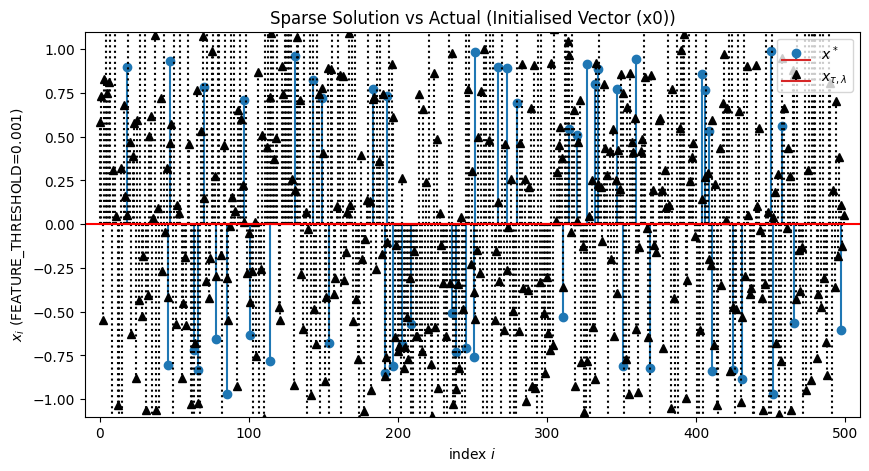
\includegraphics[scale=0.35]{outputs/part_3/initial-x}
\caption{$x_0$ vs Sparse Vector}
\label{fig:}
\end{figure}

Plotting the objective function values vs the number of iterations for both the algorithms:

\begin{figure}[h]
\centering
\begin{minipage}{.5\textwidth}
  \centering
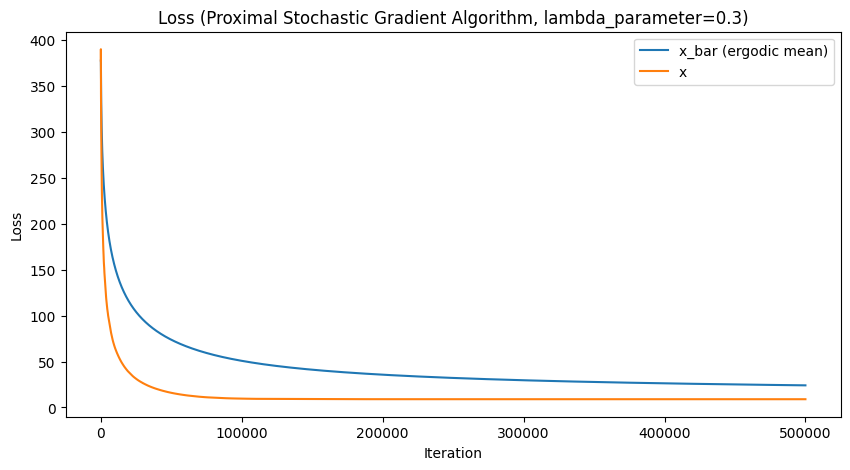
\includegraphics[scale=0.3]{outputs/part_3/psga-loss}
\caption{PSGA Loss}
\label{fig:}
\end{minipage}%
\begin{minipage}{.5\textwidth}
  \centering
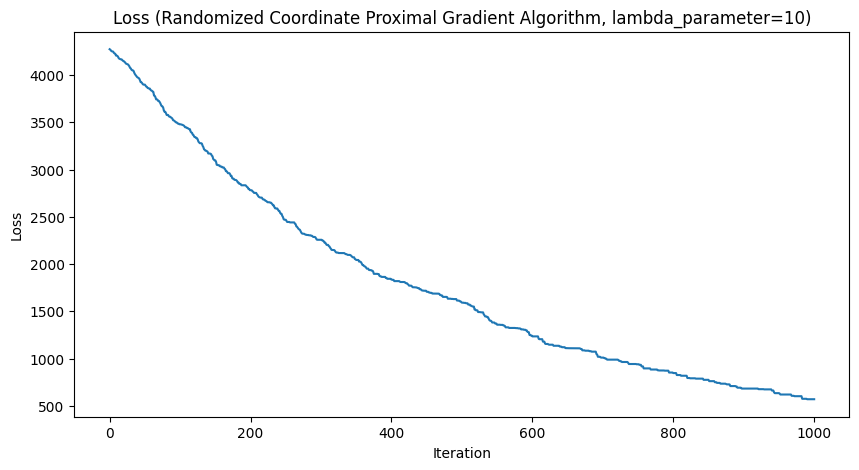
\includegraphics[scale=0.3]{outputs/part_3/rcpga-loss}
\caption{RCPGA Loss}
\label{fig:}
\end{minipage}
\end{figure}


The corresponding solution compared to the actual sparse vector for both the algorithms:

\begin{figure}[h]
\centering
\begin{minipage}{.5\textwidth}
  \centering
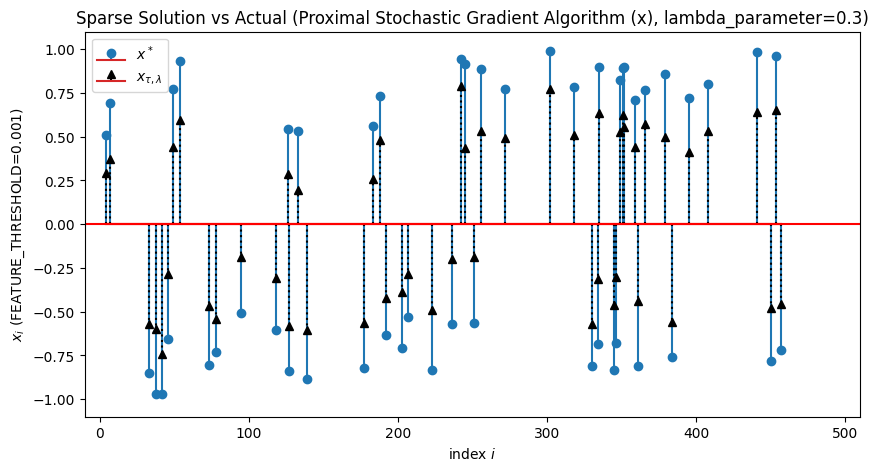
\includegraphics[scale=0.35]{outputs/part_3/psga-x}
\caption{PSGA Solution vs Sparse Vector}
\label{fig:}
\end{minipage}%
\begin{minipage}{.5\textwidth}
  \centering
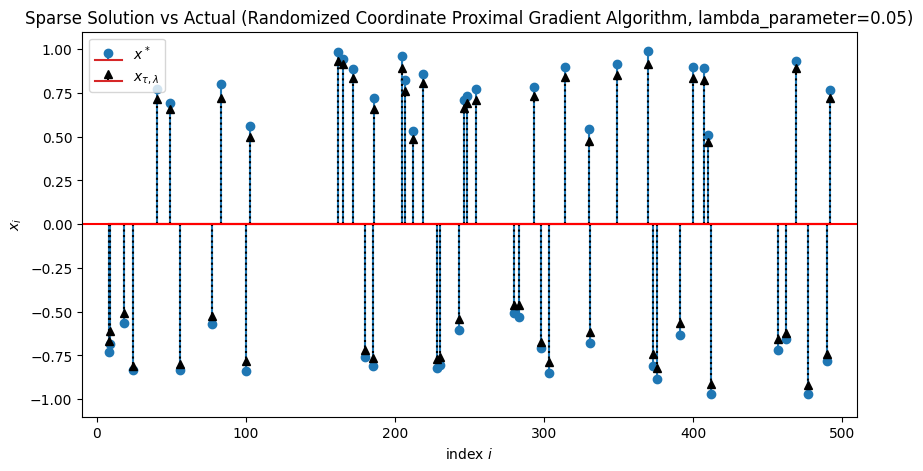
\includegraphics[scale=0.35]{outputs/part_3/rcpga-x}
\caption{RCPGA Solution vs Sparse Vector}
\label{fig:}
\end{minipage}
\end{figure}


\newpage
\section*{Part 4: Support Vector Machines}

We are given the primal problem:

\[\min_{w \in \mathcal{H}} \frac{\lambda}{n} \sum_{i=1}^{n} (1-y_i \langle w, \Lambda(x_i)\rangle)_{+} + \frac{\lambda}{2}\| w\|^2\]

We can express in the form:

\[\min_{w \in \mathcal{H}} g(w) + f(w)\]

where:

\[g(w) = \frac{\lambda}{n} \sum_{i=1}^{n} (1-y_i \langle w, \Lambda(x_i)\rangle)_{+}\]

and

\[f(w) = \frac{\lambda}{2}\| w\|^2\]

The corresponding dual problem:

\[\min_{\alpha \in \mathbb{R}^n} \frac{1}{2} \langle \mathbf{K}_y \alpha, \alpha \rangle - \langle \textbf{1}_n, \alpha\rangle + \sum_{i=1}^{n} i_{\left[0, \frac{1}{\lambda n}\right]}(\alpha_i)\]


We can express in the form:

\[\min_{\alpha \in \mathbb{R}^n} g^*(\alpha) + f^*(\alpha)\]


\subsection*{4.1}

\subsection*{4.2}

\newpage
\subsection*{4.3}

\begin{figure}[h]
\centering
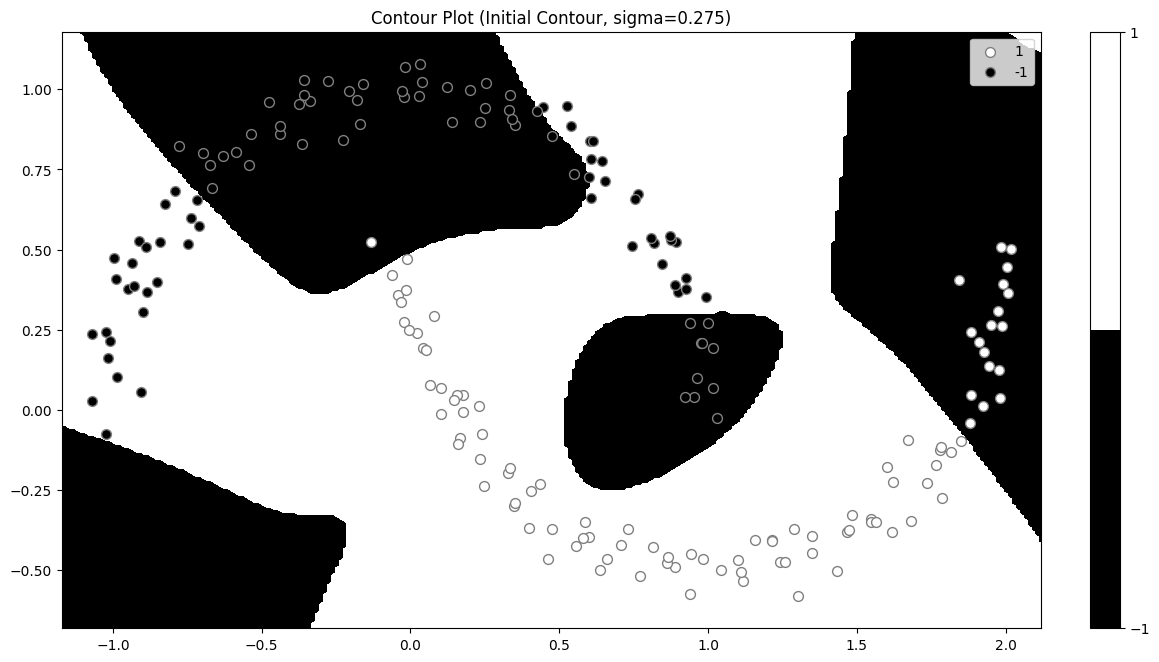
\includegraphics[scale=0.4]{outputs/part_4/initial-contour}
\caption{Initial Contour Plot}
\label{fig:}
\end{figure}


\begin{figure}[h]
\centering
\begin{minipage}{.5\textwidth}
  \centering
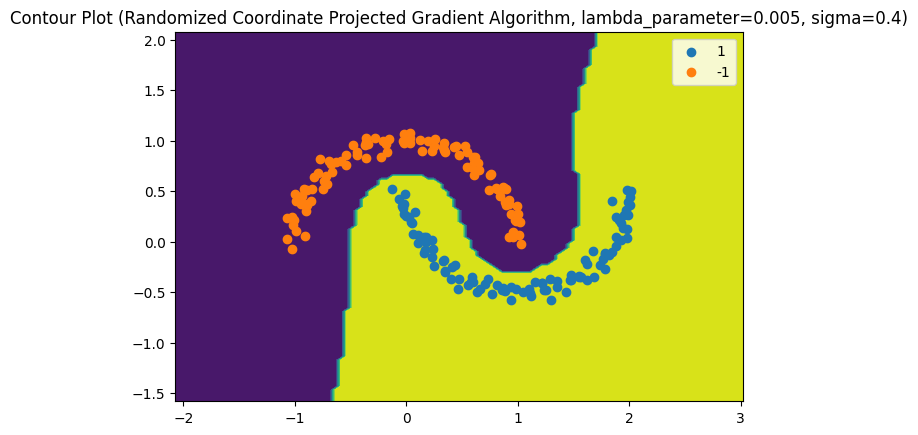
\includegraphics[scale=0.4]{outputs/part_4/rcpga-contour}
\caption{RCPGA Contour Plot}
\label{fig:}
\end{minipage}%
\begin{minipage}{.5\textwidth}
  \centering
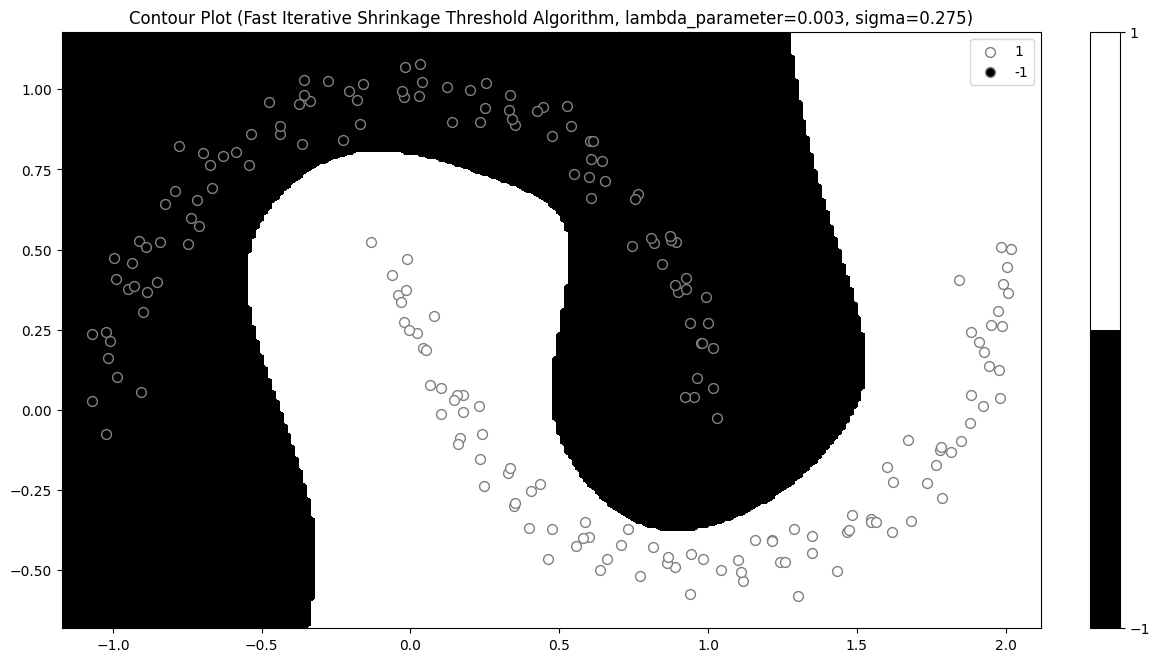
\includegraphics[scale=0.4]{outputs/part_4/fista-contour}
\caption{FISTA Contour Plot}
\label{fig:}
\end{minipage}
\end{figure}

\subsection*{4.4}

\begin{figure}[h]
\centering
\begin{minipage}{.5\textwidth}
  \centering
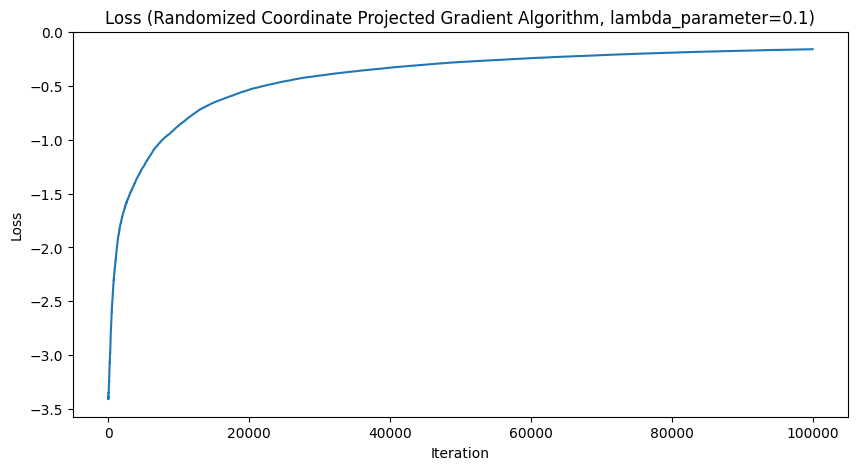
\includegraphics[scale=0.3]{outputs/part_4/rcpga-loss}
\caption{RCPGA Loss}
\label{fig:}
\end{minipage}%
\begin{minipage}{.5\textwidth}
  \centering
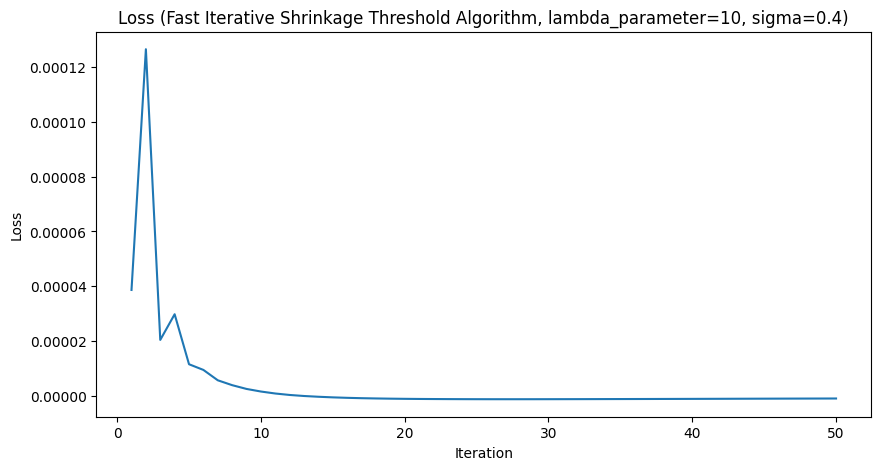
\includegraphics[scale=0.3]{outputs/part_4/fista-loss}
\caption{FISTA Loss}
\label{fig:}
\end{minipage}
\end{figure}

\end{document}
